% Use class option [extendedabs] to prepare the 1-page extended abstract.
\documentclass[extendedabs]{bmvc2k}
\usepackage[colorlinks = true,
            linkcolor = blue,
            urlcolor  = blue,
            citecolor = blue,
            anchorcolor = blue]{hyperref}
\usepackage{kotex} % 한국어 사용 가능

% Document starts here
\begin{document}
\title{RNN and LSTM}
\addauthor{
Lee Gwan Hui$^1$, \today}{}{1}
\addinstitution{
$^1$2017142136, Department of Electrical and Electronic Engineering, Yonsei University.}
\maketitle
\let\thefootnote\relax\footnote{This is an extended abstract. The full paper is available at the \href{https://github.com/LeeGwanHui/TIL/tree/main/deeplearning_ham}{github}. }
\vspace{-0.2in}
\section{개요}
 \quad 이 보고서에서는 RNN과 관련된 논문과 이를 응용한 LSTM의 블로그 글을 요약 정리할 것이다.

 \section{Recurrent neural network based language model\cite{mikolov2010recurrent}}
 \subsection{motivation}
 \quad statistical language modeling의 목표는 주어진 context를 기반으로 textual date의 다음 word를 예측하는 것이다. 
 여럽게 말했지만 간단히 말하면 '나는 연세대학교에 재학중이다.' 같은 문장에서 '나는 연세대학교에'라는 context를 기반으로 '재학중이다'를 예상하는 task이다.
 기본적으로 확률을 이용해 예측하는 모델로써 language model은 문장의 확률 또는 단어의 등장확률을 예측하는데 사용되어
 기계번역, 음성인식, 자동 완성 등에 활용될 수 있다. \cite{youtube} language model의 기본은 n-gram model이였다. 
 n-gram language model이란 Neural Network 이전에 사용되었던 Language model로 바로 다음에 올 단어을 예측하기 위해 살펴볼 
 단어의 갯수를 정하여 modeling하는 방법을 말한다. 즉 여기서 n은 앞에 몇개의 단어를 볼 것인지를 의미한다.
 \newline  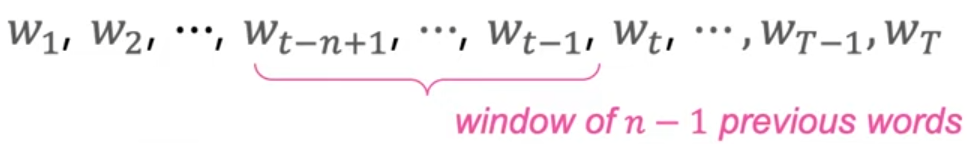
\includegraphics[width=6cm]{images/06_language.PNG}
 \newline 이런 n-gram language model의 문제점으로는 sparsity problem과 storage problem이 있었다. 먼저 sparsity problem이란 
 n이 커질수록 단어 예측 정도가 안 좋아져서 일반적으로 n<5로 설정한 모델을 말하는 것이고 storage problem이란 n이 커지거나 corpus가 증가하면서 모델의
 크기가 증가하는 문제점을 말한다. 즉 다시 말해 긴 문장으로써 다음 단어를 예상하는 경우에는 사용하기 힘들다는 단점이 있다는 것이다.
 이 논문에서는 이런 n-gram model의 한계를 뛰어넘는 Neural Network 기반의 language model을 제시한다.

 \subsection{Method}
 \quad  language modeling으로써 neural network을 사용한 최초의 모델은 Bengio가 제안하였다\cite{bengio2000neural}. Bengio가 제안한 model은 단어의 distributed representation을 
 학습하는 model이다. 
 \newline  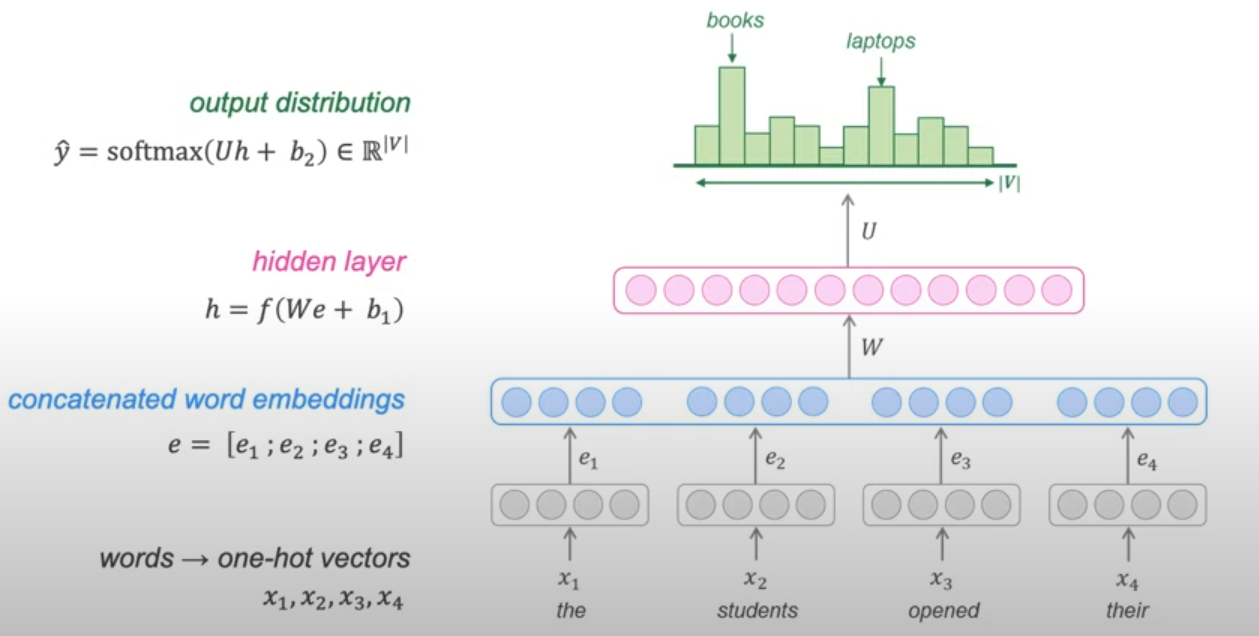
\includegraphics[width=6cm]{images/07_language.PNG}
 \newline 이 model은 fixed window 크기가 매우 작다는 window 크기의 한계가 있었다. 또한 각 word에 완전히 다른 가중치가 곱해지기 때문에
 한 문장에서 연결적인 단어들을 표현하기에는 부족했다.(no symmetry) 그래서 이 RNN 논문에서 이전에 일어난 사건을 바탕으로 현재 일어나는 사건을
 예상하는 model을 만드는 것으로 Recurrent neural network을 제안했다. 논문에서는 다른 이미지를 사용했지만 아래 이미지가 더 이해하기 쉽기 때문에 아래 그림으로
 이해해보자. 
 \newline  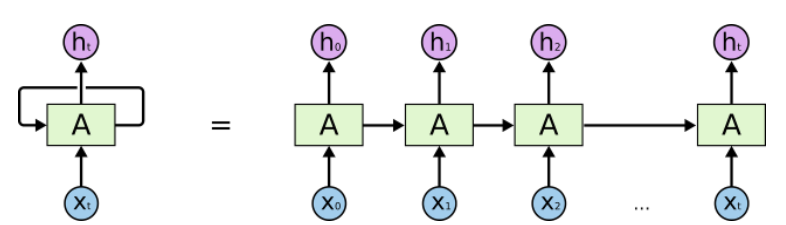
\includegraphics[width=\linewidth]{images/00_language.PNG}
 위의 그림에서 말하는 Recurrent은 위와 같이 반복되는 구조를 말한다. 이렇게 만들어진 model은 sequence와 list를 예상할 수 있다.
 \newline  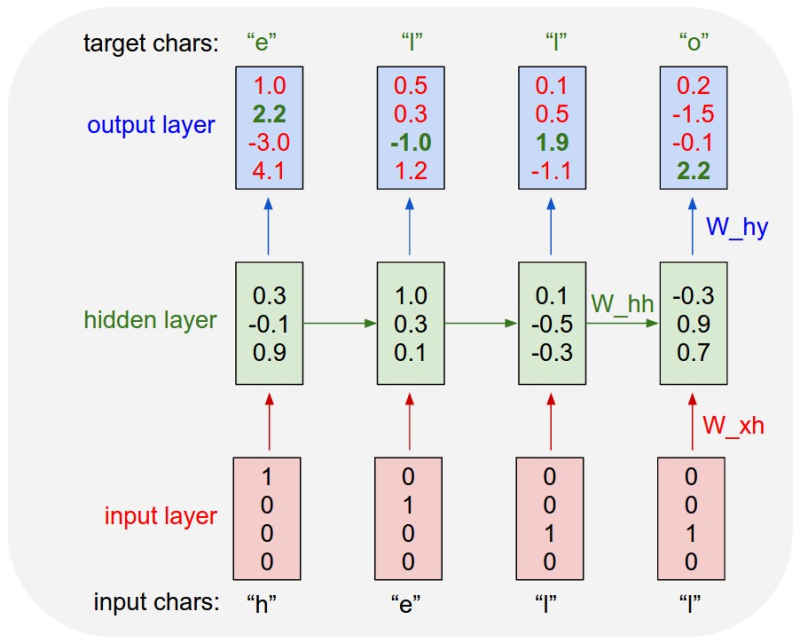
\includegraphics[width=6cm]{images/01_language.PNG}
 \newline 예시로 설명하자면 hello라는 자동 완성기능을 사용한다고 가정했을 때 위의 그림과 같이 한 알파벳이 나올때 다음 알파벳을 예상하도록 학습을 진행시켜야 한다.
 이제 다시 논문으로 돌아와서 수식으로써 위의 과정을 표현해보자. input layer을 x로 , hidden layer을 s로 output layer을 y로 표기하여
 time t에서 networ의 input을 x(t), output y(t), hidden layer은 s(t)로 표기한다고 해보자. 그럼  hidden layer의 상태가 s(t)일 때, input vector x(t)는 
 current word를 표현하는 w와 time t-1에서 context layer s의 neuron에서의 output인 s(t-1)을 concatenating하여 나타낸다.
 $$ x(t) = w(t) + s(t-1) $$
 $$ s_j(t) = f(\Sigma_i x_i(t)u_{ji})$$
 $$ y_k(t) = g(\Sigma_j s_j(t)v_{kj})$$
 위의 식에서 f(z)을 나타내고 sigmoid activation function g(z)는 softmax function을 나타낸다.
$$ f(z) = \frac{1}{1+e^{-x}}$$
$$ g(z_m) = \frac{e^{z_m}}{{\Sigma}_k e^{z_k}}$$
\newline  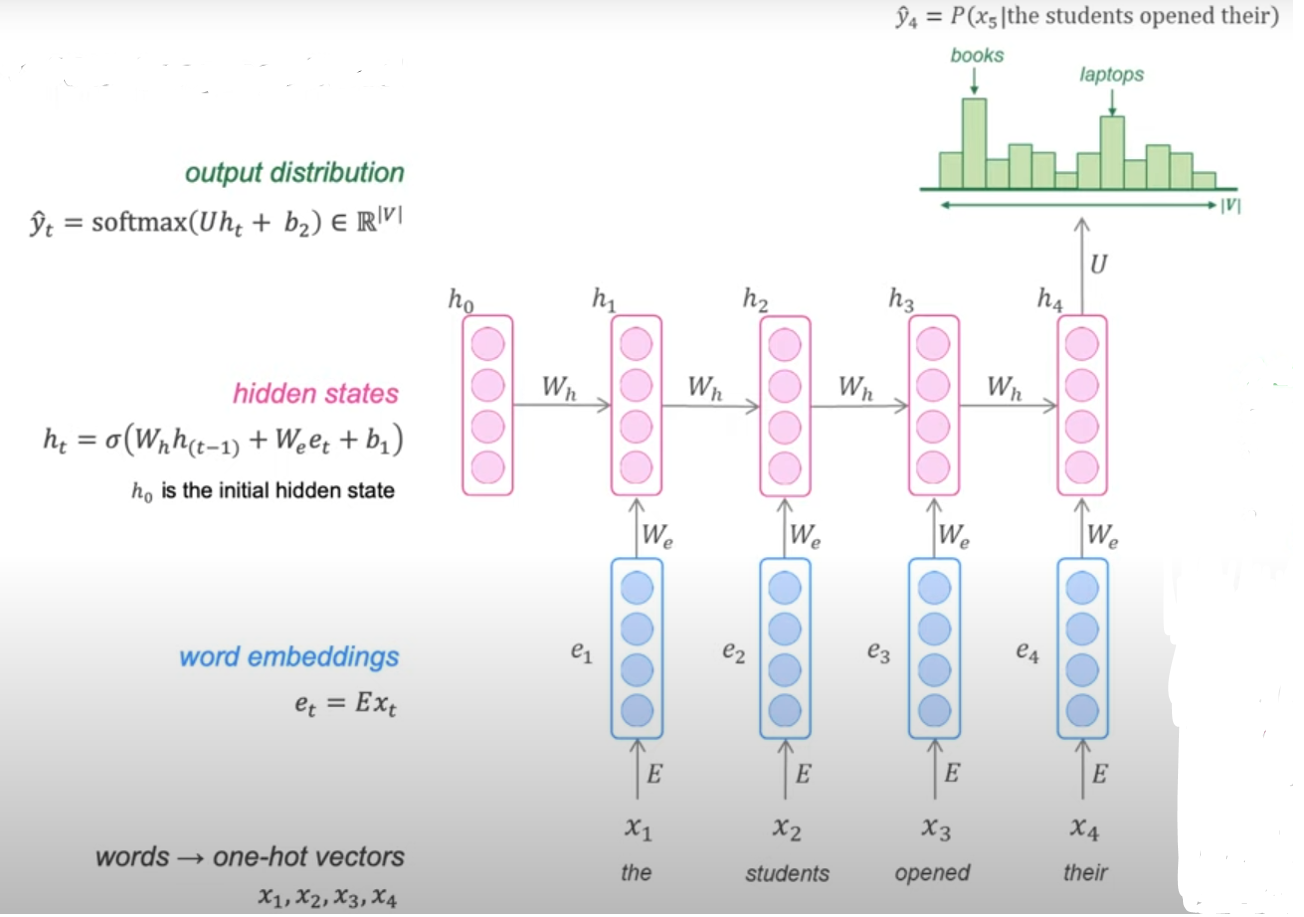
\includegraphics[width=8cm]{images/02_language.PNG}
\newline 즉 input으로 들어간 값이 layer 속에서 계속 누적되면서 확률 분포를 출력하는 구조의 layer이다.
RNN 모델의 장점으로는 input의 길이에 제한이 없고 이론적으로는 길이가 긴 timestep t에 대해 처리가 가능하다는 점과
입력에 따라서 model의 크기가 변하지 않는다는 것이다. 또한 가중치가 동일하므로 위에서 말한 n-gram에 비해 symmetry하다.
하지만 실제로 길이가 긴 time step t에 대해서 처리가 불가능하고 계산이 느리다는 단점도 존재한다.
\newline \quad training detail에 대해서 언급하자면 wight의 경우는 N(0,0.1)
Gaussian noise로 initialization 하고 SGD을 사용한다. Learning rate는 0.1을 시작으로 scheduling을 진행해주었다.
이렇게 나온 output layer y(t)는 probability distribution of next word given previous word w(t) and context s(t-1)을 표현한다.
업데이트를 위한 loss로는 Cross entropy loss 사용한다. 또한 학습방법으로 train을 할때 역시 학습을 진행하는 dynamic model을 적용한다.
이 과정을 통해 model은 new domains에서도 자동적으로 적응할 수 있다.

\subsection{Experiments}
\quad RNN을 사용하면 n-gram 기반 모델에 비해 language model의 성능 측정 단위인 perplexity가 감소하는 것을 확인할 수 있다. 
또한 아래 그림처럼 다른 모델에 비해 word Error Rate(WER) 이 감소하는 것을 볼 수 있다. 
여기서 RNN model은 6.4M word만을 학습시켰는데도 더 성능이 좋다.
\newline  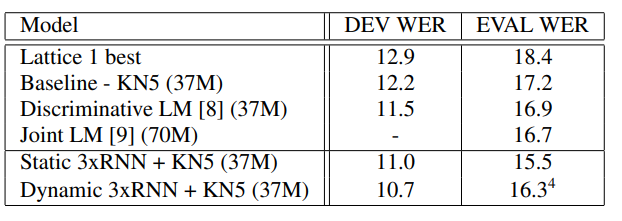
\includegraphics[width=\linewidth]{images/03_language.PNG}

\subsection{Conclusion}
\quad RNN이 기존의 n-gram 기반 language model 보다 data의 수가 적음에도 불구하고 더 좋은 성능을 보였다. 기존의 language model의 
 paradigm이였던 단지 n-grams을 발전시키고 , 더 좋은 성능을 이끌어내기 위해 새로운 training data를 사용하는 것이라는 것을 
 RNN으로써 paradigm 전환을 시킬 수 있었다는 것에 이 논문의 의의가 있다.

\section{LSTM\cite{LSTM}}
 \subsection{motivation} 
 \quad RNN의 문제점은 실제로는 Long-term 분석이 잘 되지 않는다는 것이다. 
 현재 시점의 뭔가를 예측하는 경우를 두가지로 분류하자면 첫번째는 멀지 않은 최근의 정보만 필요할 때가 있을 것이다.
 이 때는 현재를 예상하기 위해 먼 과거의 정보가 필요없기 때문에 기본적인 RNN구조로도 정확하게 예측할 수 있다.
 두번째 경우에는 먼 과거의 정보를 이용해야 정확히 현재의 정보를 예측할 수 있을때 이다. 이 때는 RNN이 실제로 잘 동작하지 않는다.
 이 블로그에서는 이 문제를 해결한 모델인 LSTM을 자세히 설명하고 있다. LSTM은 RNN를 기반하여 구조적으로 응용한 model이다.
 
 \subsection{Method}
 \quad LSTM(Long Short Term Memory networks)은 long-term dependencies의 학습이 가능하다. 
 LSTM은 long periods of time 에 대한 정보를 기억하는 것을 default behavior로 만들어졌다. 
 LSTM은 앞서 설명한 RNN과 같은 Recurrent 구조를 가지지만 반복 module간의 구조적 차이가 있다. 
 아래 그림에서 노란색 박스가 neural network layer을 나타내는데 4개의 layer가 각각 유기적으로 정보를 교환하면서
 단어를 예측하도록 설계되어 있다. 여기서 분혹색 동그라미는 pointwise operation을 의미한다.
 \newline  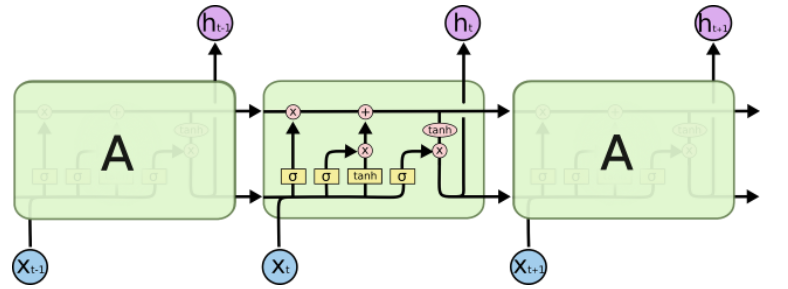
\includegraphics[width=\linewidth]{images/04_language.PNG}
 LSTM의 중요 개념은 cell state이다. 위의 그림에서는 수평 선 중에서도 위에 선을 의미한다.
 \newline  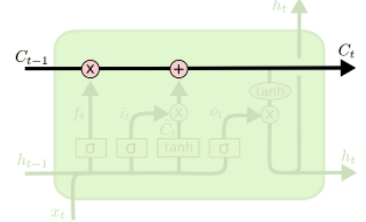
\includegraphics[width=6cm]{images/05_language.PNG}
 \newline 위의 그림의 분홍색 동그라미에서 cell state에 정보를 추가하거나 없앨 수 있다. 이를 gate라고 한다.
 먼저 x 분홍색 동그라미를 살펴보면 sigmoid output과 pointwise 곱을 진행한다.
 sigmoid의 output은 0과 1사이 값으로 각 component의 보존 정도를 결정한다. 
 \newline LSTM을 단계별로 분석하면 첫번쨰 단계는 cell state로부터 보존할 정보를 선택하는 일이다. 아래 식으로 표현할 수 있다.
 $$f_t = \sigma ( W_f \cdot [h_{t-1,x_t}] + b_f)$$
 두번째 단계는 new information 중에서 어떤 정보를 cell state에 저장할 것인지 선택하는 것이다. 
 sigmoid와 tanh가 활약하는 단계로 sigmoid는 어떤 값을 업데이트할지, tanh는 새로운 후보값 vector을 만들게 된다.
 식은 아래와 같다.
 $$ i_t = \sigma(W_i \cdot [ h_{t-1},x_t] + b_i) $$
 $$ \tilde{C_t} = tanh(W_C \cdot [h_{t-1}, x_t] + b_C)$$
 위의 값들을 이용해서 $C_{t-1}$의 값을 $C_t$로 없데이트 시켜줄 것이다. 그래서 업데이트된 $C_t$는 아래와 같이 나타낼 수 있다.
 $$ C_t = f_t * C_{t-1} + i_t * \tilde{C_t}$$
 마지막 단계는 output으로 어떤 값을 내보낼지 선택하는 일이다. 먼저 sigmoid에서 input data(word)를  cell state의 어느 부분으로 output을 내보낼 것인지 선택하고 
 cell state $C_t$를 tanh를 통과시켜서 -1과 1사이값으로 변형시켜준다음 sigmoid의 output과 pointwise 곱을 해준다. 이 방법으로 output 값이 적절히 선택 되는 것이다.
 식으로 표현하면 아래와 같다.
 $$ o_t = \sigma (W_o [h_{t-1},x_t]+b_0) $$
 $$ h_t = o_t * tanh(C_t)$$
  이과정을 주어의 예시로 이해해보자. 예를 들어 영어문장을 쓸 때 주어가 중요하다. 왜냐면 주어에 따라서 
 동사의 형태가 변할 수 있기 때문일 뿐만 아니라 나중에 나올 대명사 역시 주어에 기반하여 쓸 수 있기 때문이다. 하지만 만약 문장이
 끝났다면 이전에 저장되어 있던 주어의 정보는 더이상 가지고 있을 필요가 없다. 이 모든 과정이 위에서 단계 1,2,3으로 표현한 것과 같다.
 1번 단계에서 새로운 주어가 들어왔으므로 기존의 주어 정보를 버리고, 2번 단계에서 새로운 주어정보를 업데이트 시켜준다. 그리고 마지막 3번 단계에서 적절한
 output을 보내주는 것이다.

 \subsection{Experiments}
  이 글에서 추가적으로 LSTM의 다양한 변형들에 대해 소개한다. peephole connection을 추가한 모형이 있는데 이는 gate layer이 cell state의 값도 참고한다는 의미이다.
  Forget gate을 추가한 모델도 있는데 이는 새로운 정보가 들어가는 자리만 정보를 없애고 업데이트해준다. 또한 cell state와 hidden state을 합치고
  forget gate를 추가한 GRU model도 있다. 이같은 LSTM 모델들을 순차적으로 예상해야 하는 문제에 적절히 작용하고 RNN에 비해 성능이 좋다. 

 \subsection{Conclusion}
\quad 이 블로그의 글은 LSTM의 직관적인 이해를 돕도록 쓰여 있다. 이 글에서 밝히길 language model이 RNN으로 big step을 하였고 또한 RNN이 LSTM으로 변환되면서
또 big step이 일어났다. 그리고 다음 step으로는 attention이 매우 중요할 것이라 예상한다. attention은 RNN의 각 단계 별로 얻는 정보를 기반으로 더 큰 정보의 set를 보고 학습하는 방법이다.

\newpage
\bibliography{egbib}

\end{document}